\documentclass[11pt]{article}
\usepackage[margin=1in]{geometry}
\usepackage{graphicx}
\usepackage{booktabs}
\usepackage{amsmath}
\usepackage{natbib}
\usepackage{hyperref}
\usepackage{setspace}
\onehalfspacing

\title{Compression, Volatility, and the Limits of Small-Cap Options: \\
A Pre-Registered Empirical Investigation}
\author{Aarav Aguru \\ Kelley School of Business, Indiana University}
\date{\today}

\begin{document}
\maketitle

\begin{abstract}
This paper documents a sequence of five pre-registered empirical tests on U.S. small- and mid-cap equities (CRSP size deciles 6--8, 2015--2025), each gated by a strict development/holdout split committed before data contact. Two tests of short-horizon price reversal, unconditional and volume-conditioned, are rejected: net alpha after transaction costs is significantly negative in both cases ($t = -5.04$ and $t = -4.68$), and a pre-registered gross-return exhibit shows the second signal carried no factor-adjusted edge even before costs ($t = -1.46$). A separate hypothesis, that abnormally low trading volume forecasts elevated forward realized volatility, is confirmed in both the development sample (Newey-West $t = -6.88$) and a single, non-repeated holdout pass ($t = -3.39$), and survives a sector-relative reformulation tested the same way (dev $t = -7.02$, holdout $t = -3.06$). A subsequent attempt to monetize this forecasting relationship through short-dated equity options is rejected: using OptionMetrics contract-level quotes rather than the smoothed volatility surface, the strategy's gross-of-friction edge (+3.85\% per trade) is roughly an order of magnitude smaller than the median observed bid-ask spread (18.8\% of mid), producing a significantly negative net result ($t = -5.01$). The paper's contribution is not a trading strategy but a demonstration that a statistically real and twice-confirmed forecasting relationship need not be economically exploitable, and a worked example of how that gap can be measured directly rather than assumed.
\end{abstract}

\section{Introduction}
A substantial literature documents that recent losers among small, illiquid stocks earn positive abnormal returns over short subsequent windows. The usual explanation is compensation for liquidity provision: in names where arbitrage capital is scarce or costly to deploy, someone must absorb selling pressure, and that service is paid for \citep{nagel2012, avramovchordiagoyal2006}. A separate concern cuts against this. Published anomalies tend to weaken after publication, as the trading required to exploit them competes away the return that described them \citep{mcleanpontiff2016}. Both observations motivate the same practical question for a researcher approaching this literature fresh: does a reversal signal, built carefully and tested honestly on a recent sample, still work, or has it already been absorbed into how the market prices small-cap risk?

This paper answers that question and then follows the answer where it leads. Two reversal specifications are tested; both fail, and the way they fail is informative. The raw returns these strategies earned were not evidence of mispricing but passive exposure to a published short-term reversal factor, which means nothing about them was ever novel. That result motivated a different question about the same universe: whether small-cap stocks carry information not about the direction of future price movement but about its magnitude. They do, and the relationship survives both an out-of-sample test and a reformulation designed to strip out sector-level effects. The paper then documents an attempt to convert that forecasting result into a tradeable position, an attempt that fails for a specific and measurable reason rather than an ambiguous one.

Every hypothesis below was pre-registered. The universe definition, signal construction, holding period, cost assumption, gate criterion, and holdout window were fixed and committed to version control before the relevant data was loaded, and the commit hash for each phase is cited in the section that reports it. Where a design was later revised, the revision appears as a new phase document rather than an edit to the old one. This discipline is not incidental to the results. Two of the five phases produced numbers that would have been easy to improve by adjusting a parameter after the fact, and the pre-registration is what makes the reported failures interpretable as evidence rather than as an unlucky draw from a search that continued until something worked.

\section{Data and Methodology}
\subsection{Data Sources}

Equity data comes from CRSP daily files covering 2015 through 2025, including price, return, volume, shares outstanding, and delisting information. Point-in-time universe membership is constructed from CRSP's own classification fields rather than a static ticker list, so a stock enters and exits the sample on the dates it actually met the criteria. Factor returns for risk adjustment come from the Ken French data library: the five-factor model \citep{fama2015}, momentum, and the short-term reversal factor. Industry classification comes from Compustat's GICS fields, linked to CRSP through the CRSP/Compustat Merged linking table. Options data comes from OptionMetrics IvyDB US, in two forms whose difference turns out to matter: the standardized volatility surface, which reports model-fitted premium at fixed tenor and delta grid points, and the option price file, which reports actual quoted bid and ask for individual traded contracts.

\subsection{Universe Construction}

The universe is NYSE size deciles 6 through 8, assigned monthly using NYSE-only breakpoints in the Fama-French convention and applied to all NYSE, AMEX, and NASDAQ listings. Decile assignment uses month $t-1$ data and applies throughout month $t$, so no forward-looking information enters the membership decision. Filters restrict to ordinary common shares priced at or above \$5 at assignment, excluding REITs, ADRs, and closed-end funds. Monthly universe size ranges from 913 to 1,341 names with a mean of 1,038, and no month deviates more than 30\% from its trailing twelve-month mean.

\subsection{Testing Protocol}

The sample is split once, permanently, into a development window (2015--2021) and a holdout window (2022--2025). All specification decisions were made using development data only. The holdout is evaluated once per phase, after a development pass has been logged, and is never re-run, re-tuned, or re-split regardless of outcome. Scripts that touch holdout data are separate files from those that touch development data, and the development scripts contain no code path to the holdout window at all; this is enforced structurally rather than by convention.

Two testing frameworks appear in the paper, and the distinction matters for how the results should be read. Directional return hypotheses (Sections 3 and 6) are evaluated as alpha claims: daily portfolio returns net of costs are regressed on the five Fama-French factors plus momentum and short-term reversal, with Newey-West standard errors at ten lags, and the claim is the regression intercept. Forecasting hypotheses (Section 4) are evaluated as information-coefficient claims using a Fama-MacBeth procedure: a cross-sectional regression is run each trading day, and the resulting time series of daily coefficients is tested with the same Newey-West correction. A forecasting result establishes that one variable predicts another. It does not establish that the prediction can be traded, and the paper is careful not to conflate the two.

\subsection{Data Quality Issues Encountered}

Four data problems were identified during construction, each of which would have corrupted downstream results silently.

The Ken French factor files initially downloaded as daily series were, on inspection of the raw file headers, monthly data for two of the three files. A daily regression run against monthly factors produces no error and returns plausible-looking coefficients with badly understated standard errors. The files were re-pulled and the incorrect versions quarantined with a naming convention that preserves their provenance.

CRSP's SIC code field uses zero as a missing-value sentinel rather than null, concentrated on delisting-adjacent rows. Treated naively, roughly 17,000 stock-days would have been assigned to a nonexistent industry.

Compustat's GICS classification, as delivered through both the company names file and the CCM link table, is backfilled: zero of 15,326 tested company identifiers show a sector change across sixteen years of rows, despite GICS having undergone documented sector restructurings during that period. This means the classification available reflects each company's current sector applied retroactively, which introduces a mild look-ahead. True point-in-time GICS history was not accessible through the available subscription. Section 4's sector-relative test accordingly discloses this as a pre-registered limitation rather than correcting for it after the fact.

OptionMetrics uses the CUSIP value 99999999 as a placeholder for unidentified and synthetic instruments, shared across roughly 1,900 security identifiers. Joining on CUSIP without excluding this sentinel would have introduced index products and structured instruments into an equity-only sample.
\section{Phase R1/R2: Small-Cap Reversal}
\subsection{R1: Unconditional Reversal}

The first specification ranks stocks by trailing five-day return within the size-6-to-8 universe and holds the bottom decile long for five trading days, implemented as five overlapping daily tranches so that one fifth of capital rotates each day. Entry is at the next day's open. Costs are 15 basis points per side, with realized annualized one-way turnover of 50.4 times. The pre-registration fixed all of these parameters, along with a pass criterion requiring a positive intercept with a $t$-statistic of at least 2.0, before any return data was examined.

The gate result is a decisive rejection. Net of costs, the strategy's daily excess return is $-7.45$ basis points ($t = -5.04$), which annualizes to roughly $-18.8\%$. The regression coefficients explain why. The portfolio loads heavily on the published short-term reversal factor ($\beta = 0.562$, $t = 6.85$), on size ($\beta = 1.094$, $t = 20.84$), and on the market ($\beta = 0.969$, $t = 28.02$), producing an $R^2$ of 0.904. Whatever positive raw return this strategy generated came from exposures that are already available, already documented, and already priced. The strategy is a repackaging of ST\_Rev with a turnover cost attached.
\begin{figure}[htbp]
    \centering
    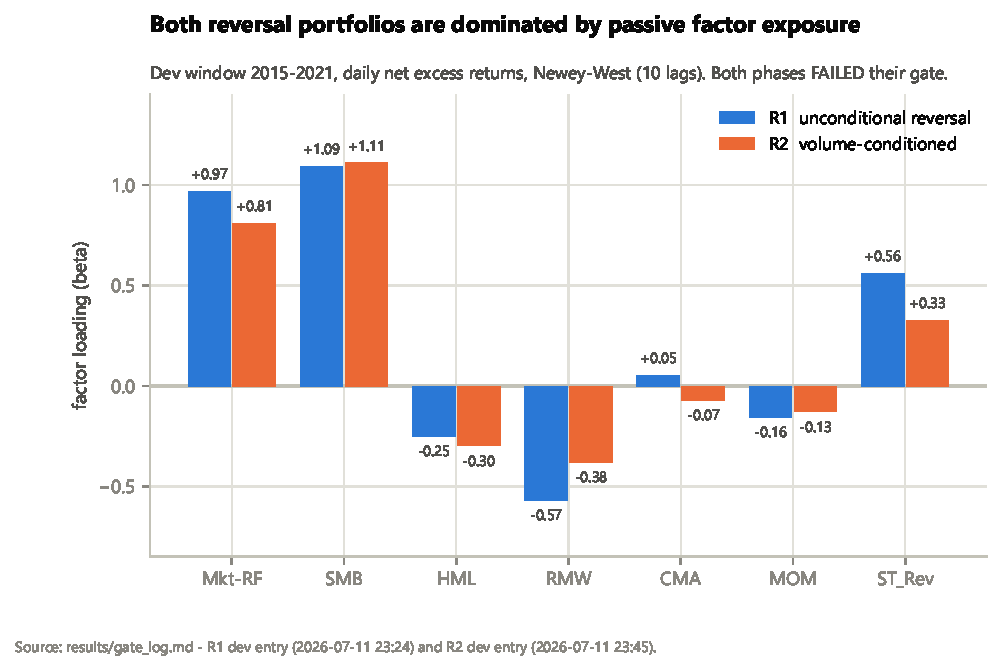
\includegraphics[width=0.85\textwidth]{results/figures/fig1_r1_r2_factor_loadings.pdf}
    \caption{Factor loadings for R1 (unconditional reversal) and R2 
    (volume-conditioned). The volume condition reduces the short-term 
    reversal loading from 0.562 to 0.326, confirming the filter selected 
    a materially different portfolio rather than a smaller version of 
    the same one. Neither specification produced factor-adjusted alpha.}
    \label{fig:factor-loadings}
\end{figure}

A pre-registered horizon exhibit, computed at one, three, and ten day holding periods and carrying no gate authority, shows the cost problem clearly. Net alpha improves monotonically as the holding period lengthens, from $-90.6\%$ annualized at a one-day hold to $-10.9\%$ at ten days, because turnover falls faster than the signal decays. No horizon in the tested range is profitable.

\subsection{R2: Volume-Conditioned Reversal}

The second specification tests whether the reversal premium concentrates in a subset of losers rather than existing uniformly across them. The economic hypothesis is that price declines accompanied by unusually heavy trading are more likely to reflect forced or panicked selling, and therefore genuine overreaction, than declines that occur on thin volume. The condition requires that the worst single day within the five-day lookback window carried dollar volume at least twice its own trailing twenty-day average. Dollar volume is used rather than share volume specifically because share counts change mechanically with splits, which would produce false spikes.

The filter behaved as designed. It reduced the candidate pool from roughly 103 names per day to 24.4, and it selected genuinely different stocks rather than a random subset: the reversal-factor loading fell from 0.562 to 0.326 and $R^2$ from 0.904 to 0.778. Four days in the seven-year sample produced no qualifying candidate at all, and the pre-registered rule holding those tranches in cash was applied without exception.

The result is another rejection, and a more informative one. Net alpha is $-8.71$ basis points per day ($t = -4.68$). More importantly, a pre-registered gross-return exhibit computing the identical regression before any transaction cost gives an intercept of $-2.72$ basis points per day with $t = -1.46$, which is statistically indistinguishable from zero. This rules out the interpretation that a real edge was destroyed by frictions. There was no factor-adjusted edge to destroy. Whatever the volume condition selected for, it was not compensated return, and the conclusion holds across every horizon tested, including a twenty-day hold whose annualized cost drag is only 3.8\%.

Two pre-registered nulls on the same mechanism, tested with different specifications and reaching the same conclusion by different routes, is the point at which continuing to search would stop being research. The reversal line closed here.
\section{Phase V1/V2: Volatility Compression as a Forecasting Signal}
\subsection{V1: Own-History Compression}

The reversal results ruled out directional prediction in this universe. They said nothing about whether the same stocks carry information about the magnitude of future movement, which is a different claim with a different economic basis. Volatility clustering is among the most replicated findings in empirical finance, and it does not require any market inefficiency to hold. If quiet periods systematically precede active ones, that is a forecasting relationship, not an arbitrage opportunity, and it should be testable without the arbitrage-decay concerns that motivated Section 3.

The compression score for each stock-day is the ratio of its trailing twenty-day mean dollar volume to its trailing sixty-day mean, both computed with a one-day lag. A low ratio means recent activity has fallen below the stock's own longer-run baseline. Stocks are ranked cross-sectionally into deciles each day, with decile 1 the most compressed. The forecast target is annualized realized volatility over the following ten trading days, and the test is a Fama-MacBeth cross-sectional regression of forward volatility on compression decile, with the daily coefficient series tested using Newey-West standard errors at ten lags. Because this is an exploratory forecasting test without an attached cost model, the pre-registration set a higher bar than the alpha claims: $|t| \geq 3.0$ rather than 2.0.

The development result clears that bar by a wide margin. Across 1,718 daily cross-sectional regressions, the mean coefficient is $-0.004265$ with $t = -6.883$, and the coefficient is negative on 72.8\% of trading days. The holdout, evaluated once, is sign-consistent at $-0.003348$ ($t = -3.385$ for the record; the pre-registered criterion was sign consistency alone). The out-of-sample coefficient retains roughly 79\% of the development magnitude, which is the kind of moderate attenuation a real effect produces when it moves to unseen data, rather than the collapse toward zero that overfitting produces.

The decile table complicates the interpretation in a way worth reporting rather than smoothing over. Forward volatility declines monotonically from decile 1 (0.466) through decile 8 (0.389), exactly as hypothesized, and decile 1 is the sample maximum. But decile 10, the most expanded names, is the second highest at 0.432. The relationship is U-shaped, not linear. This is economically sensible: compressed stocks are more likely to move because quiet precedes activity, and expanded stocks are more likely to move because volatility clusters and recent activity persists. Both tails carry information. The pre-registered linear specification passes because the compression side dominates, but the compression tail is the novel finding here, and the expansion tail is a restatement of volatility clustering that required no new signal to discover. The holdout reproduces the same shape, with decile 1 at 0.515 and decile 10 at 0.490, confirming the pattern is structural rather than sample-specific.
\begin{figure}[htbp]
    \centering
    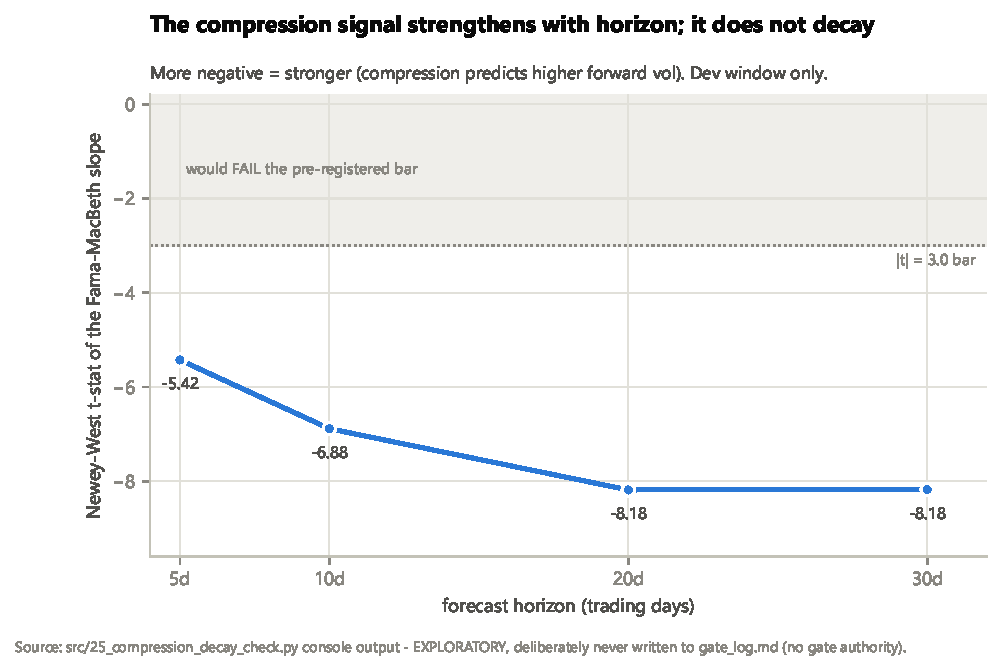
\includegraphics[width=0.8\textwidth]{results/figures/fig3_v1_decay_curve.pdf}
    \caption{Newey-West $t$-statistic on the compression coefficient by 
    forecast horizon, development window. The signal strengthens rather 
    than decays with horizon, which is what permits the thirty-day 
    option tenor in Section 6 without extending beyond validated 
    forecasting range. Exploratory exhibit, no gate authority.}
    \label{fig:decay}
\end{figure}
\subsection{V2: Sector-Relative Compression}

A stock can appear quiet relative to its own history simply because its entire sector has gone quiet. V2 tests whether removing that common component sharpens the signal. The construction subtracts, from each stock's compression ratio, the same-day median compression ratio among other in-universe stocks in its GICS sector, requiring at least twenty qualifying stocks per sector-day. The static-GICS limitation described in Section 2 applies and was pre-registered before testing.

The result passes both gates with a marginally stronger $t$-statistic than V1 (dev $t = -7.016$ versus $-6.883$; holdout $t = -3.062$) and a slightly smaller coefficient. The honest reading is that the two signals are close to equivalent. Sector-relative compression is own-history compression minus a common term, and if most of the compression signal is stock-specific rather than sector-driven, subtracting the sector median changes the ranking very little. What V2 establishes is that the V1 result is not an artifact of sector-level volatility cycles. What it does not establish, because it was not tested, is whether sector adjustment adds information beyond V1; a joint specification with both variables was never pre-registered and is left as an open question.

\subsection{Horizon Behavior}

A separate exploratory check, carrying no gate authority, extended the forecast target to five, twenty, and thirty trading days. The signal does not decay with horizon. The Newey-West statistic strengthens from $-5.43$ at five days to $-6.88$ at ten and $-8.18$ at both twenty and thirty. This is consistent with compression predicting a persistent shift in volatility regime rather than a transient burst, and it is also mechanically expected in part, since longer realized-volatility windows are less noisy targets and permit more precise coefficient estimation. The finding matters for Section 6, where instrument availability forces a thirty-day tenor and this exhibit establishes that the signal has not weakened at that horizon.
\begin{figure}[htbp]
    \centering
    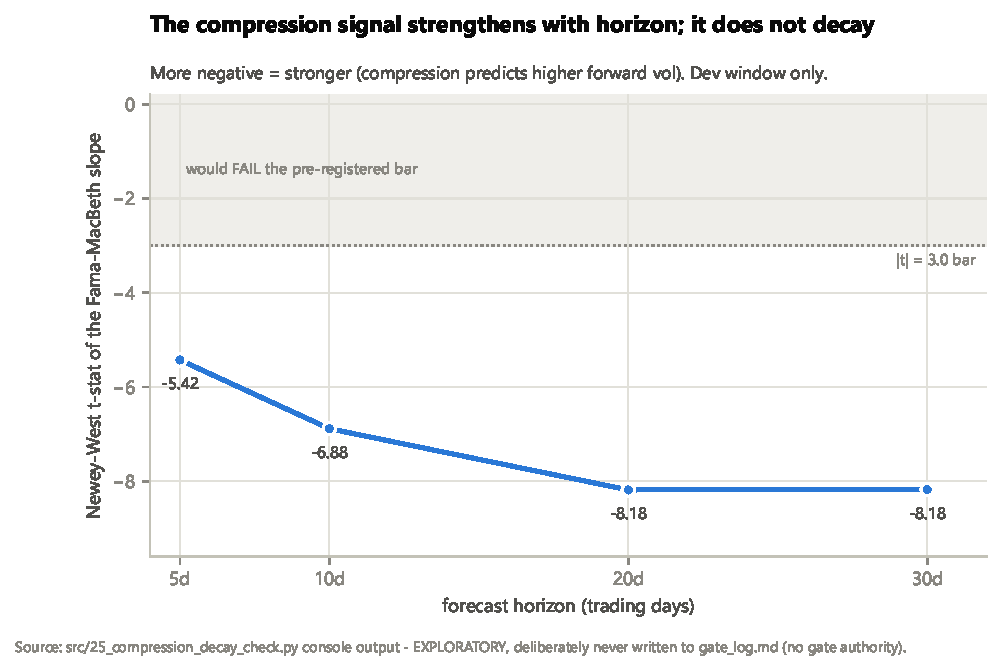
\includegraphics[width=0.8\textwidth]{results/figures/fig3_v1_decay_curve.pdf}
    \caption{Newey-West $t$-statistic on the compression coefficient by 
    forecast horizon, development window. The signal strengthens rather 
    than decays with horizon, which is what permits the thirty-day 
    option tenor in Section 6 without extending beyond validated 
    forecasting range. Exploratory exhibit, no gate authority.}
    \label{fig:decay}
\end{figure}
\section{Phase K0: Forecaster Selection}
The compression signal establishes that quiet stocks subsequently move more than active ones on average. It does not, on its own, produce a point forecast of how much a specific stock will move, which is what any options-based expression requires. Selecting that forecaster is itself a specification decision capable of being optimized after the fact, so it was pre-registered as a separate phase with a fixed evaluation metric and a fixed decision rule before any candidate was run.

Three forecasters competed on development-window data over a common sample of 1,557,783 stock-days, evaluated by mean absolute error against realized ten-day forward volatility. Trailing twenty-day realized volatility, a parameter-free estimate, achieved an MAE of 0.1751. A per-stock GARCH(1,1) achieved 0.1810. Using each compression decile's average forward volatility as a categorical forecast achieved 0.1980. The simplest candidate won outright, and the pre-registered tie-breaking rule favoring simplicity was not needed.
\begin{figure}[htbp]
    \centering
    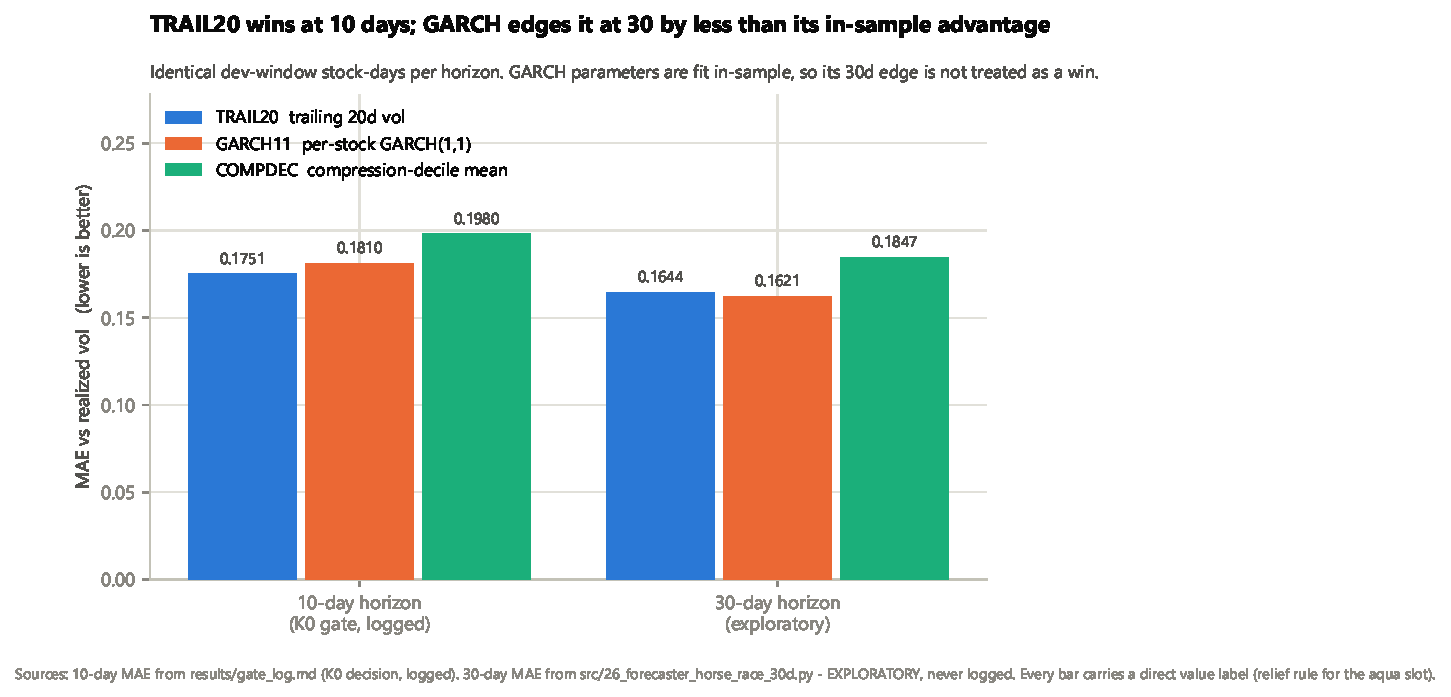
\includegraphics[width=0.8\textwidth]{results/figures/fig4_k0_horse_race.pdf}
    \caption{Mean absolute forecast error by candidate forecaster at 
    ten- and thirty-day horizons. Trailing twenty-day volatility wins 
    outright at ten days and loses narrowly at thirty, by a margin 
    smaller than GARCH's in-sample fitting advantage plausibly accounts 
    for. The thirty-day comparison is exploratory and carries no gate 
    authority.}
    \label{fig:horserace}
\end{figure}

The GARCH result deserves comment because its loss is more meaningful than the margin suggests. GARCH was fit on the same development window against which it was scored, giving it an in-sample advantage that trailing volatility, having no fitted parameters, does not receive. It lost anyway. It also failed to converge or produce a usable fit for roughly 12\% of stocks, which in a coverage-constrained universe is a real cost rather than a technical footnote.

An exploratory re-run at the thirty-day horizon, prompted by the tenor constraint discovered in Section 6, reverses the ranking narrowly: GARCH achieves 0.1621 against trailing volatility's 0.1644. The reversal is economically interpretable, since mean reversion toward each stock's unconditional volatility level matters more at longer horizons and GARCH models that decay explicitly while a trailing average extrapolates flat. But the 1.4\% relative margin is smaller than GARCH's in-sample advantage plausibly accounts for, and the coverage cost remains. Trailing twenty-day volatility was retained as the sanctioned forecaster on that basis, with the reasoning documented before Section 6 was run rather than after its result was known.
\section{Phase K1: Attempting to Monetize the Signal}
\subsection{Design}

Sections 4 and 5 establish a forecasting relationship and a forecaster. Neither says anything about whether the options market already prices the same information. Testing that requires taking a position whose payoff depends on realized movement exceeding what the market charges for it, and the natural instrument is a straddle: simultaneous long call and long put at the same strike, profitable when the underlying moves substantially in either direction.

The pre-registration fixed the following before any options data was joined. Candidates are V1 decile-1 stock-days. Entry occurs when the theoretical straddle value implied by the trailing-twenty-day volatility forecast exceeds the observed market price by at least 25\%, a threshold derived from a quantity known before the entry rule was written: matched-sample mean implied volatility (0.6105) exceeded V1 decile-1 mean realized volatility (0.4656) by roughly 23.7\%, indicating a structural volatility risk premium in these names, and the threshold was set slightly above that figure so the rule demands more edge than the average headwind rather than merely matching it. Positions are held ten trading days, the horizon on which the underlying signal was gated, then closed. Overlapping positions on the same underlying are permitted and no cap on concurrent positions applies, both fixed in advance.

Tenor was set at thirty days rather than ten for two independent reasons that point the same direction. Coverage: near-the-money implied volatility in this universe is concentrated at the thirty-day tenor, with roughly 90.6\% of valid surface points there against 9.4\% at ten days, because small-cap names rarely have listed expirations close to ten days out. Signal: the horizon exhibit in Section 4 established that compression's forecasting power does not weaken at thirty days. Neither reason depends on knowing the result.

\subsection{Two Reconstructions and Their Failure}

The initial implementation used OptionMetrics' volatility surface, which was the data available at the time. The surface reports fitted premium at standardized constant-maturity points and contains no bid or ask. This creates a problem specific to the exit. A position entered in a thirty-day option and held ten trading days is, at exit, a straddle with roughly fifteen calendar days remaining, and the surface does not report a price for that instrument. It reports the price of a fresh thirty-day straddle on that date.

Valuing the exit at the fresh thirty-day price implicitly assumes the position lost no value to time decay over the holding period. That implementation produced a mean per-trade return of $+9.96\%$ and an apparent gate pass at $t = +5.381$. The result is an artifact. An at-the-money straddle's time value scales approximately with the square root of remaining tenor, so a straddle with fifteen days left is worth roughly 73\% of an otherwise identical thirty-day straddle, and omitting that decay inflates every exit.

A second implementation corrected for this by scaling the exit implied volatility by $\sqrt{T_{\text{remaining}}/30}$. This overcorrected. Black-Scholes evaluated at fifteen days already applies the correct time scaling for a given volatility; discounting the volatility input as well double-counts the decay. That implementation produced $-11.74\%$ per trade and a gate failure at $t = -10.179$. It is also economically backwards in direction, since short-tenor implied volatility after a volatility event typically exceeds thirty-day implied volatility rather than falling 28\% below it.

The two estimates bracket a value neither can measure. The 21.7 percentage point swing between them matches the square-root-of-time arithmetic almost exactly, which confirms the diagnosis but does not resolve the question. Both entries remain in the project's gate log rather than being deleted, since the sequence is the evidence that the final estimate was not selected from among alternatives after the fact.
\begin{figure}[htbp]
    \centering
    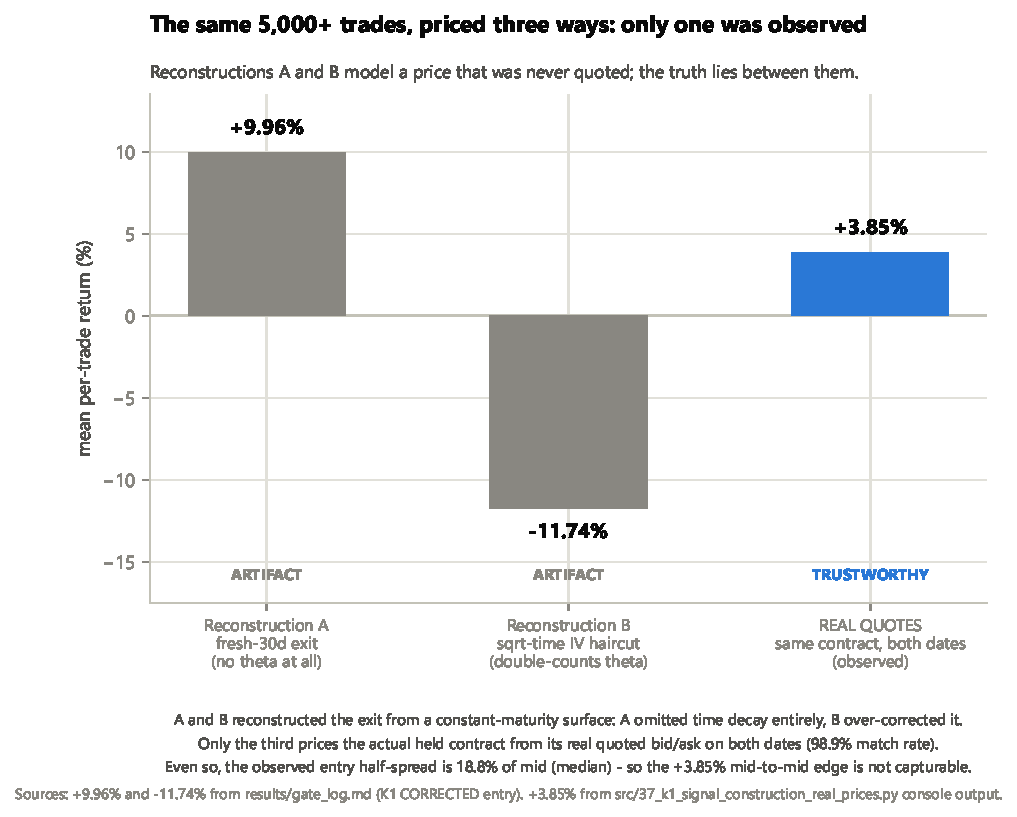
\includegraphics[width=0.85\textwidth]{results/figures/fig5_k1_three_valuations.pdf}
    \caption{Three estimates of K1's mean per-trade return. The two 
    reconstructions bracket the value measured from matched contract 
    quotes, in the directions predicted by their respective biases: 
    omitting time decay overstates, double-counting it understates. 
    Only the third is an observed price.}
    \label{fig:three-valuations}
\end{figure}

\subsection{Resolution with Contract-Level Quotes}

OptionMetrics' option price file reports actual quoted bid and ask for individual contracts, identified by a unique contract identifier that persists across dates. Matching each trade's entry and exit to the same contract by that identifier eliminates the reconstruction entirely: the exit price is the quoted price of the instrument actually held, on the date actually held to. Of 5,416 locked trades, 5,356 (98.9\%) found both an entry and an exit quote; the remaining 60 were excluded and counted rather than estimated.

The mid-to-mid mean per-trade return is $+3.85\%$. It falls between the two reconstructions, closer to the optimistic one, consistent with the direction and approximate magnitude of the bias each introduced. This is the paper's best estimate of the strategy's gross-of-friction edge, and taken alone it looks encouraging.

The same data shows why it is not tradeable. The median entry-side bid-ask spread on these contracts is 18.8\% of mid price, and the mean is 29.8\%. Roughly half of matched contract-days carry zero volume and zero open interest, and 23\% have no bid at all. A round-trip position crossing that spread on entry and exit must gain on the order of 40 to 60\% before it breaks even, against an edge of 3.85\%. The daily portfolio return, aggregating overlapping positions with spread cost applied to both legs, is $-72.14$ basis points ($t = -5.011$), and only 31.6\% of trading days are positive. 
\begin{figure}[htbp]
    \centering
    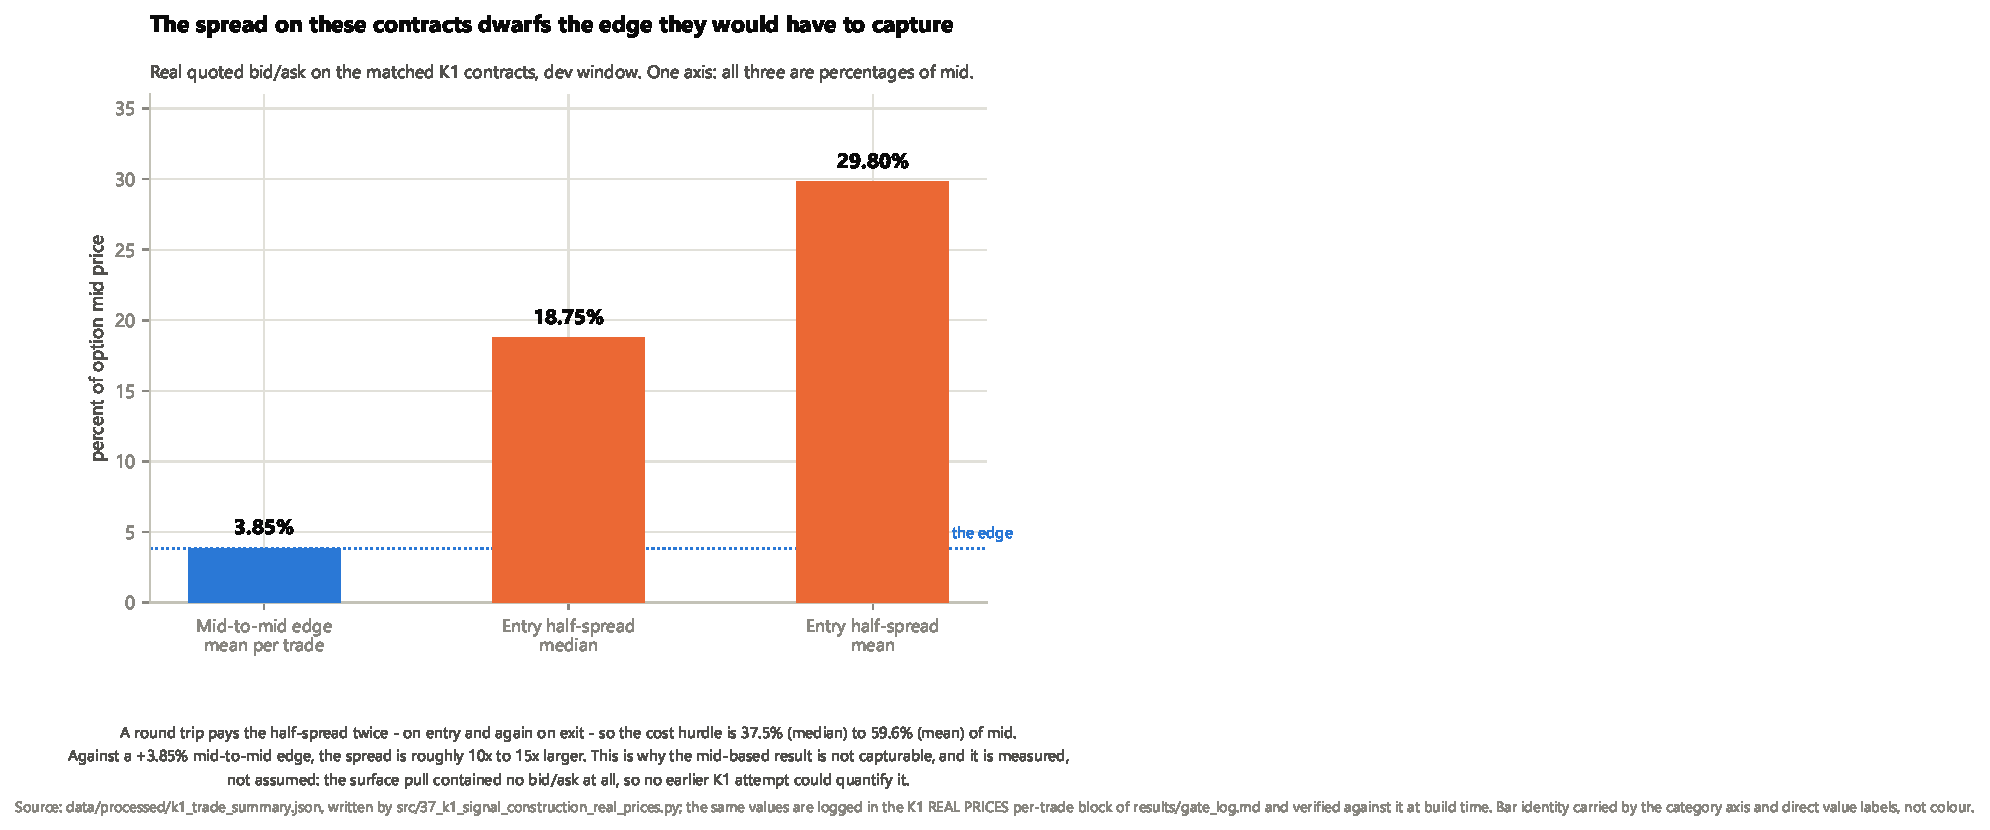
\includegraphics[width=0.8\textwidth]{results/figures/fig6_k1_spread_vs_edge.pdf}
    \caption{The measured gross edge (+3.85\%) against the measured 
    round-trip cost of transacting, computed from matched contract-level 
    bid/ask quotes: a straddle crosses the spread on both entry and 
    exit, so the true breakeven hurdle is 37.5\% of mid at the median 
    spread and 59.6\% at the mean, roughly ten to fifteen times the 
    edge itself.}
    \label{fig:spread-vs-edge}
\end{figure}

Four diagnostic views, all pre-registered without gate authority, confirm the result is not an artifact of any single period or filtering choice. Excluding 2020 makes it worse ($t = -5.813$), so the 44\% of trades concentrated in that year are not driving the failure. Restricting to contracts with nonzero volume or open interest does not help ($t = -5.004$). And under the worst realistic fill assumption, buying at the ask and selling at the bid rather than transacting at mid, the strategy loses 1,053 basis points per day and is positive on 0.7\% of days.

The finding is not that the volatility forecast is wrong. Sections 4 and 5 establish that it is right, twice, out of sample. The finding is that the instrument available to express it cannot be transacted in at prices resembling those a model would show, and that the gap between the model price and the transactable price is roughly an order of magnitude larger than the edge itself.
\section{Discussion}

The results separate cleanly into two claims that are easy to conflate and important to keep apart.

The first is that short-horizon reversal in this universe, tested both unconditionally and with a volume condition designed to isolate forced selling, produces no factor-adjusted edge. The R2 gross-return exhibit is the strongest single piece of evidence here, since it shows the absence of edge before any cost assumption enters. Whatever premium existed in this mechanism historically appears to have been absorbed into the published short-term reversal factor, which is consistent with the post-publication decay documented by \citet{mcleanpontiff2016}, though this paper cannot distinguish decay from the possibility that the premium never existed net of realistic frictions in this particular size range.

The second is that volume compression predicts forward realized volatility, robustly, and that the relationship survives an out-of-sample test, a sector-relative reformulation, and horizon extension to thirty days. This is a forecasting result, and the paper is deliberate about not calling it more than that. The U-shape in the decile tables indicates the linear specification understates what is happening: the compressed tail is the novel finding, the expanded tail restates volatility clustering, and a specification treating them as distinct signals would likely be sharper. That specification was not pre-registered and therefore was not tested.

The third result is the one with the most transferable lesson. A statistically real forecasting relationship, confirmed out of sample, produced a positive gross edge in the instrument designed to express it, and still failed by a wide margin because the bid-ask spread in that instrument exceeds the edge by roughly a factor of ten. The failure is not statistical but structural, and it was invisible in the smoothed volatility surface data, which reports a fitted price where no transactable price exists. The three-attempt sequence in Section 6 illustrates a general risk in derivatives research: model-reconstructed prices can be wrong in either direction, by amounts that exceed the effect being measured, and the direction of the error is not always obvious in advance.

\section{Limitations}

Sector classification is backfilled rather than point-in-time, as described in Section 2. Section 4's V2 result therefore contains a mild look-ahead in sector membership, disclosed in the pre-registration before testing rather than discovered afterward.

Transaction cost modeling in Sections 3 and 6 differs in kind. The equity strategies assume a flat 15 basis points per side, which is a reasonable but unverified approximation. The options results use observed quoted spreads, which is stronger, but include no commission model; per-contract commissions would add further drag, meaning the reported options results are an upper bound on realizable performance rather than a conservative estimate.

The options sample ends 2025-08-29 rather than 2025-12-31, following the data's actual coverage. Options coverage of the decile-1 universe is uneven by size, at 90.8\%, 87.8\%, and 78.7\% for deciles 6, 7, and 8 respectively, so the traded universe in Section 6 tilts slightly larger than the universe on which the signal was gated.

Each holdout was evaluated exactly once and cannot be re-examined. This is a feature of the design rather than an oversight, but it does mean that questions raised by a holdout result cannot be answered within the same phase.

Section 6's trade count is concentrated: 44\% of qualifying trades fall in 2020. The pre-registered diagnostic splits show the failure is not driven by that concentration, but the sample is less evenly distributed across market regimes than the seven-year window suggests.

Finally, the V1 and V2 signals are close enough in construction that the paper cannot claim sector adjustment adds independent information. Establishing that would require a joint specification, which was not pre-registered and is left open.

\section{Future Directions}

The finding that transaction costs dominate the identified edge does not imply the forecast is unmonetizable in principle. It implies that the specific instrument and trade structure tested here cannot express it. Three directions follow.

The first is to abandon the derivatives expression entirely and use the volatility forecast as a position-sizing overlay on the underlying equity, in the manner of volatility-managed portfolios \citep{moreiramuir2017}: reduce exposure to names forecast to become volatile, increase it in names forecast to remain quiet. This trades the underlying rather than its options, avoiding the spread problem that ends Section 6, at the cost of converting an alpha claim into a risk-adjustment claim.

The second is to test whether the signal aggregates. The 2020 concentration in Section 6 suggests the compression signal captures something partly systematic rather than purely idiosyncratic. If small-cap compression broadly forecasts small-cap volatility broadly, the aggregated signal might transfer to index-level volatility instruments, where spreads are measured in single-digit percentages rather than the 18.8\% median observed here.

The third is to restructure when the spread is paid. The current design crosses the bid-ask twice, on entry and exit. Holding to expiration rather than closing early would incur the spread once, since settlement requires no transaction, at the cost of holding beyond the horizon on which the signal was validated. Whether the edge survives that extension is an empirical question requiring its own pre-registration.

A fourth direction, outside what this paper can test, concerns execution. A participant quoting inside the spread rather than crossing it as a taker faces a fundamentally different cost structure than the one modeled here. Whether the identified edge is accessible to a liquidity provider in these contracts, as opposed to a liquidity taker, cannot be determined from historical quote data alone and would require order-level modeling that the available data does not support.

\bibliographystyle{apalike}
\bibliography{references}

\appendix
\section{Full Gate Log}
The complete gate log, containing all ten pre-registered evaluations in 
chronological order with full regression output, diagnostic exhibits, 
and disclosed bias statements, is maintained in the project repository 
at \url{https://github.com/gurud0x/driftfire_rerun/blob/main/results/gate_log.md}. 
Each entry records the phase, the governing pre-registration document 
and its commit hash, the evaluation window, the decision, and any 
limitations disclosed at the time of running. Entries are appended and 
never overwritten; the two superseded K1 evaluations discussed in 
Section 6 remain in place above the final one.

All pre-registration documents are in \texttt{docs/}, and the commit 
hash cited in each phase section can be verified against the repository's 
commit history to confirm the document predates the corresponding 
analysis.

\end{document}